
\begin{figure}[htbp]
    \centering

    \begin{subfigure}[b]{0.88\textwidth}
        \centering
        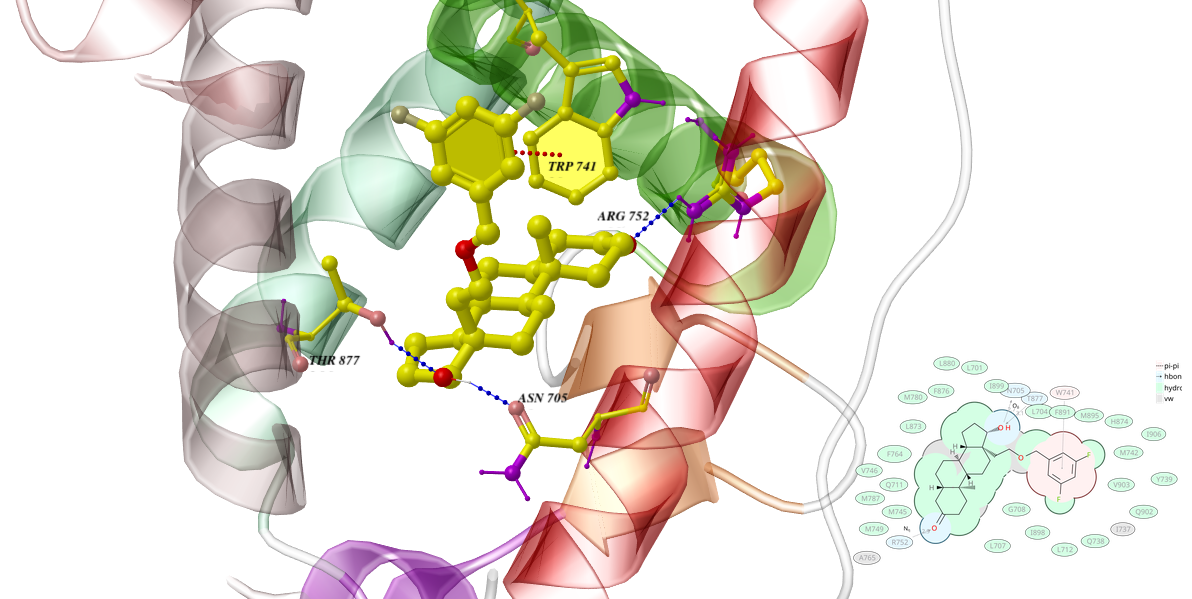
\includegraphics[width=\textwidth]{AR/combined/enm_2pnu.png}
        \caption{ENM (yellow) in the 2PNU AR conformation.}
        \label{fig:ar-enm}
    \end{subfigure}

    \vspace{0.8cm}

    \begin{subfigure}[b]{0.88\textwidth}
        \centering
        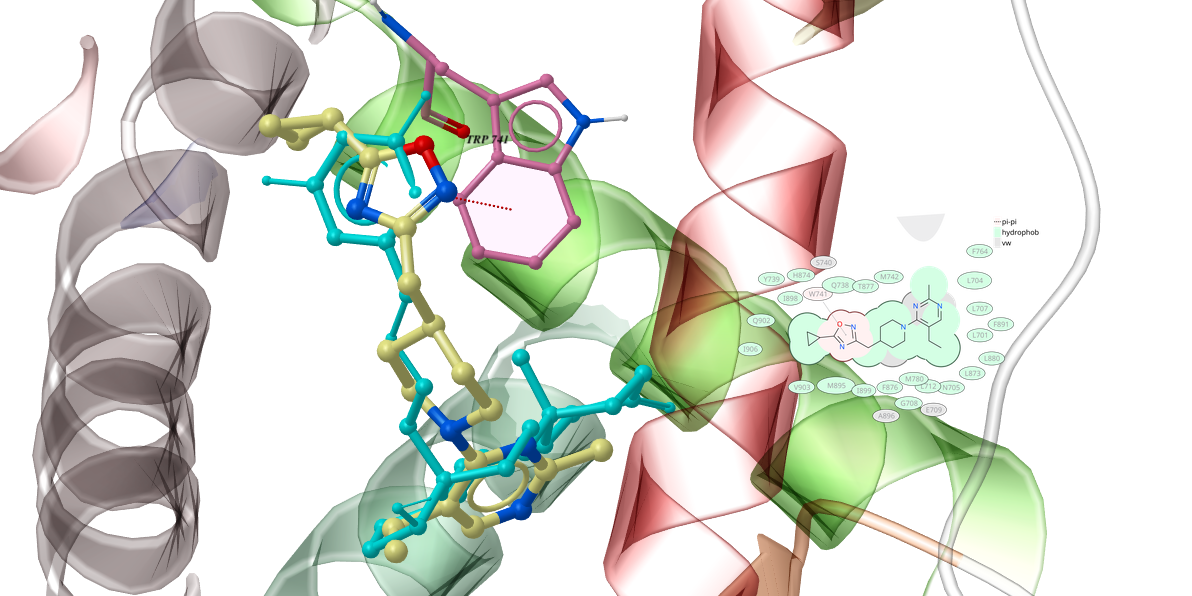
\includegraphics[width=\textwidth]{AR/combined/enm_sup_a.png}
        \caption{Compound 681 (yellow) superimposed with ENM (blue).}
        \label{fig:ar-681-superimposition}
    \end{subfigure}

    \vspace{0.8cm}

    \begin{subfigure}[b]{0.88\textwidth}
        \centering
        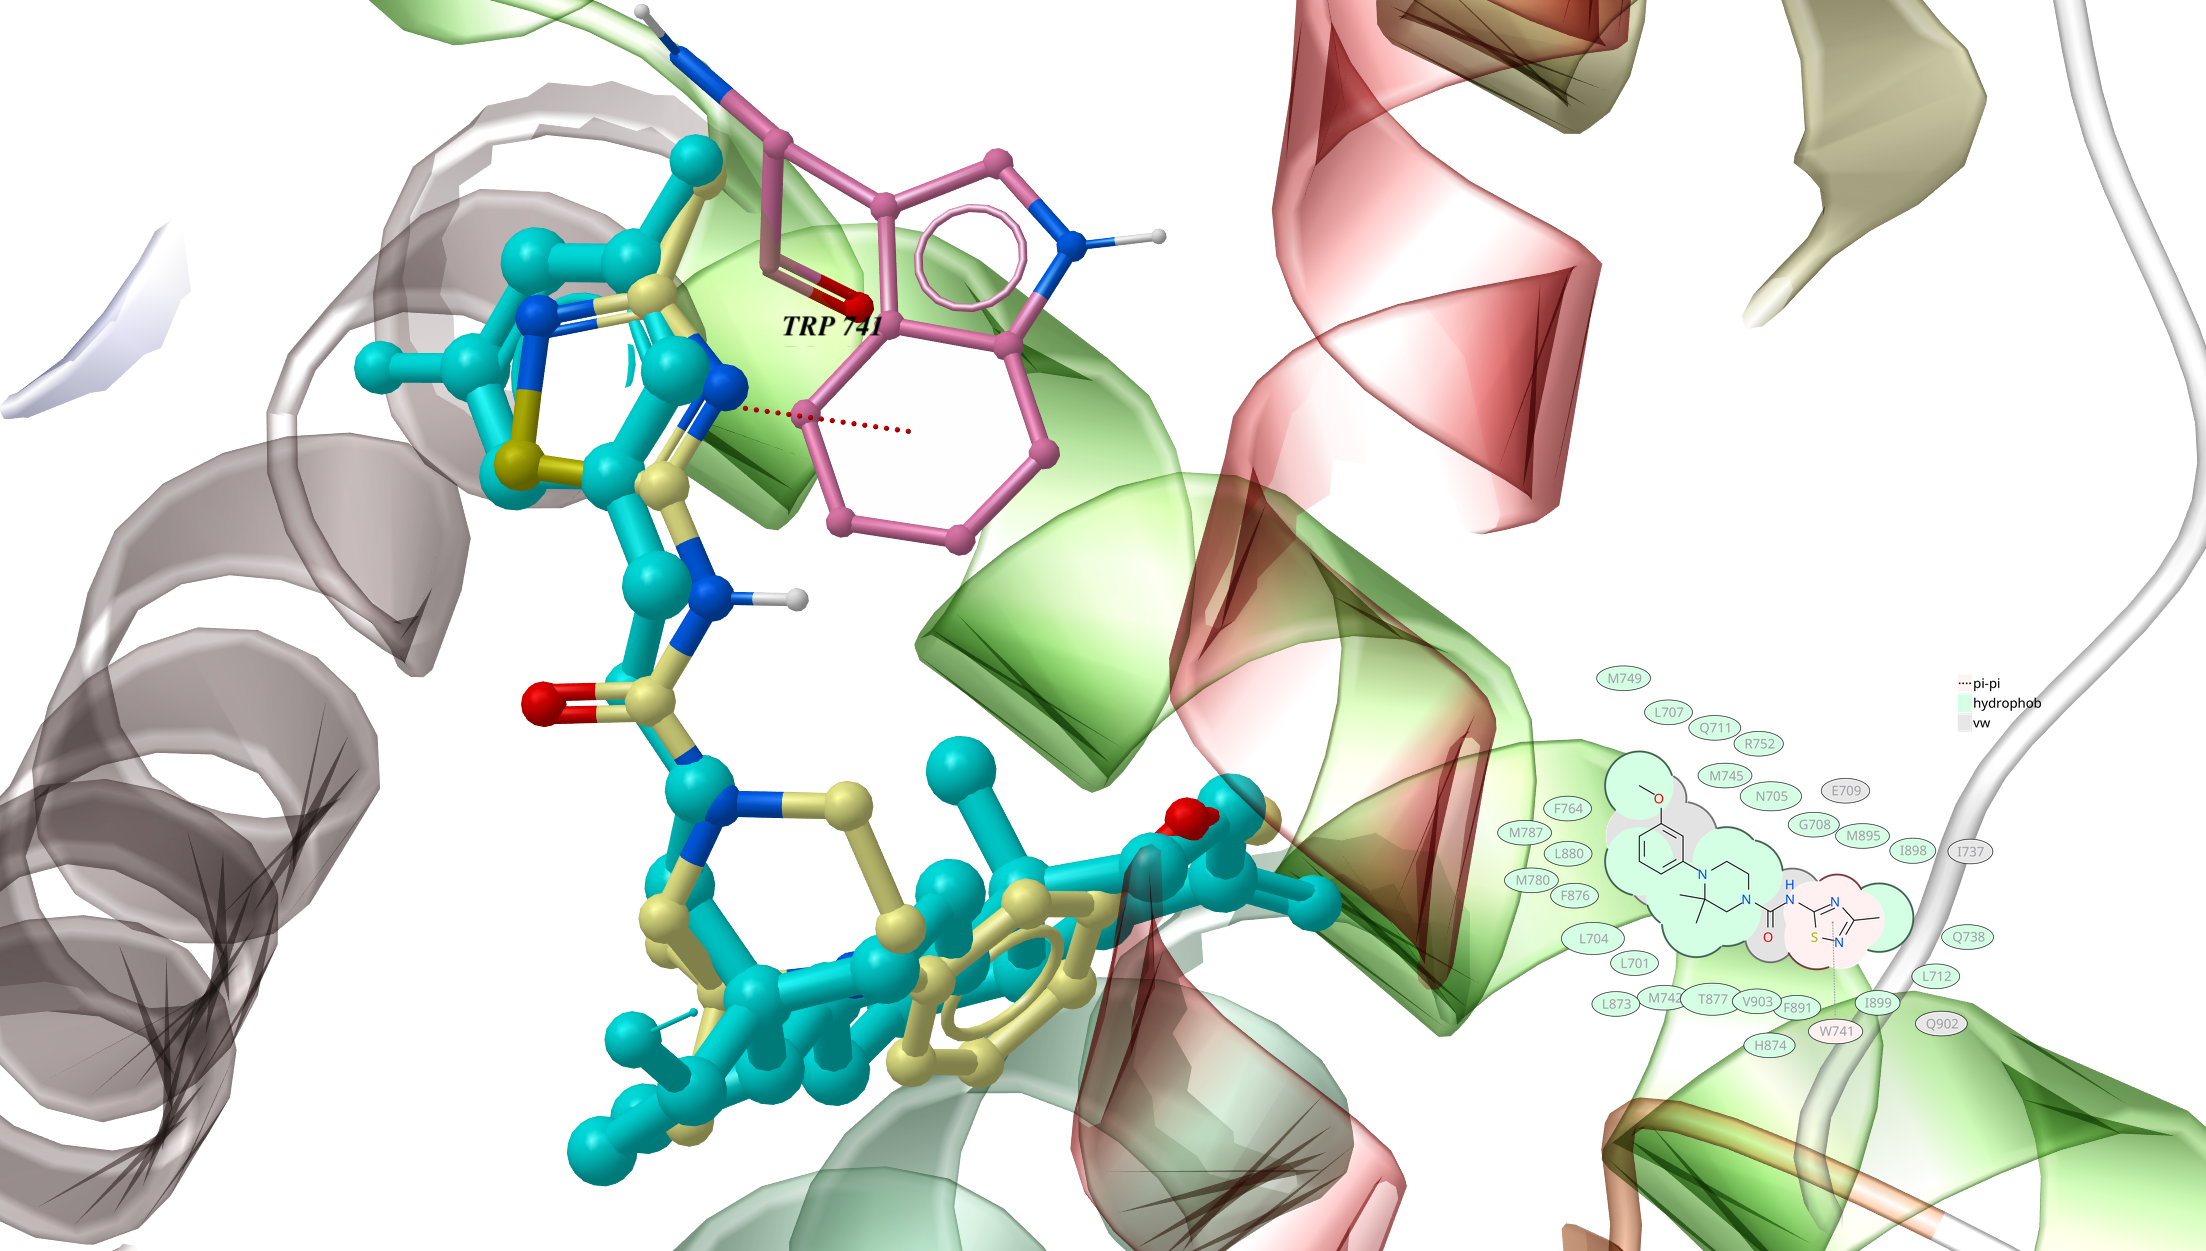
\includegraphics[width=\textwidth]{AR/combined/enm_sup_b.png}
        \caption{Compound 889 (yellow) superimposed with ENM (blue).}
        \label{fig:ar-889-superimposition}
    \end{subfigure}

    \caption{Visual comparison of predicted AR binding poses in the 2PNU receptor conformation. Hydrogen bonds are represented by blue dashed lines, whereas $\pi$--$\pi$ interactions are represented by red lines. The corresponding 2D interaction diagram is displayed at the bottom right of each 3D binding-pose view.}
    \label{fig:ar-interaction-analysis}
\end{figure}